\documentclass[10pt]{scrbook}
\usepackage[utf8]{inputenc}
\usepackage{listings} % for listings, of course ;-)
\usepackage{amssymb}
\usepackage{graphicx} % for \includegraphics
\lstset{language=C++}
\author{Wolfgang Keller}
\title{Documentation of 101\_browser}
\begin{document}
\maketitle
\tableofcontents

\part{Introductory material}

\chapter{FAQ}

\paragraph{What will make 101\_browser special?}

There are lots of existing browsers around. Why would you need another one?
\begin{itemize}
\item Current web browsers tend to get optimized for consuming and not for adding abilities to hack or reverse-engineer websites. Especially in areas of analyzing downloaded binary files (most browsers rely on external libraries there). So there is a gap to fill.
\item Wolfgang Keller does not believe that the browser vendors put enough emphasis on security and privacy. It is planned (if time allows) to do correctness proofs of critical parts. Additionally sometimes it is approved to risk security holes for compliance with outdated websites (for example: content negotiation or cross-side Javascript). 101\_browser will break standards in these cases (but in a very well-documented way, so that web developers won't have to fear of "`another browser hell"')
\item Many different standards (HTML+JS, PDF, SWF) tend to converge in delivered features. Why not write the browser as a unified runtime engine for all of them?
\end{itemize}

\paragraph{Where does the name "`101\_browser"' come from?}

Originally Wolfgang Keller called the browser project "`x\^{}2+1"' (he likes naming his projects after mathematical objects -- especially at this time). Where does this strange name come from?

Consider the field of real numbers $\mathbb{R}$. As you learn in any introductory course about abstract algebra for this field there exists (up to isomorphism) only one non-trivial algebraic field extension, which is isomorphic to $^{\mathbb{R}[x]}/_{\left\langle x^2+1\right\rangle}$, where $\left\langle x^2+1\right\rangle$ -- of course -- denotes the ideal generated by $x^2+1$.

This field extension is -- of course -- isomorphic to the field of complex numbers.

If you look back into mathematical history the discovery of the complex numbers lead to a mathematical breakthroughs. I only say "`fundamental theorem of algebra"' and "`complex analysis"' (which is a lot more elegant than "`standard calculus"' ;-) ). Since I think browser technology needs a radical breakthrough of disruptive changes Wolfgang Keller found it a fitting name. ;-)

Unluckily the project server of the university which he used at the beginning did not like the \^{} character in its name -- so he was requested to change the project name. Since he wanted to preserve the spirit of the name he chose the coefficient order of the polynomial $x^2+1$ which obviously is 1, 0, 1 and renamed it to 101\_browser.

\paragraph{What does the "`MTAx"' namespace mean?}

Since "`101"' is not a valid namespace in C++, "`MTAx"' was used, which is "`101"' encoded in Base64.

\chapter{Principles of 101\_browser}

\section{Avoid lookup tables}

Although some algorithms can be made faster by using lookup tables, we try to avoid to make use of them since they add additional complexity.

\section{Use as few additional libraries as possible}

For many features there are existing libraries. But in 101\_browser we avoid to make use of them. Why?

\begin{itemize}
\item You never know how well they are maintained
\item It is a goal of 101\_browser to provide an \emph{independent} implementation of web standards (this implies that it hopefully doesn't have \emph{the same} security bugs as in the commonly used implementation)
\item Since it should be easy to add support for experimental features, we can make our own implementation very similar in style -- this makes them easier to learn if you have already read into other parts of the source code
\end{itemize}

So: when is it OK to use an existing library?
\begin{itemize}
\item It has to be cross-platform
\item It has to be widely used
\item If it is an abstration of platform-specific details it should be the most low-level abstration that is available
\end{itemize}
At the time of writing (26th of December 2010) only the Standard library of C/C++ and OpenGL are accepted in this topic. Despite zlib is still used, it is planned to replace it by an own implementation soon.

\part{User documentation}

\part{Reference documentation}

\chapter{Parts of 101\_browser}

\section{Geolocation}

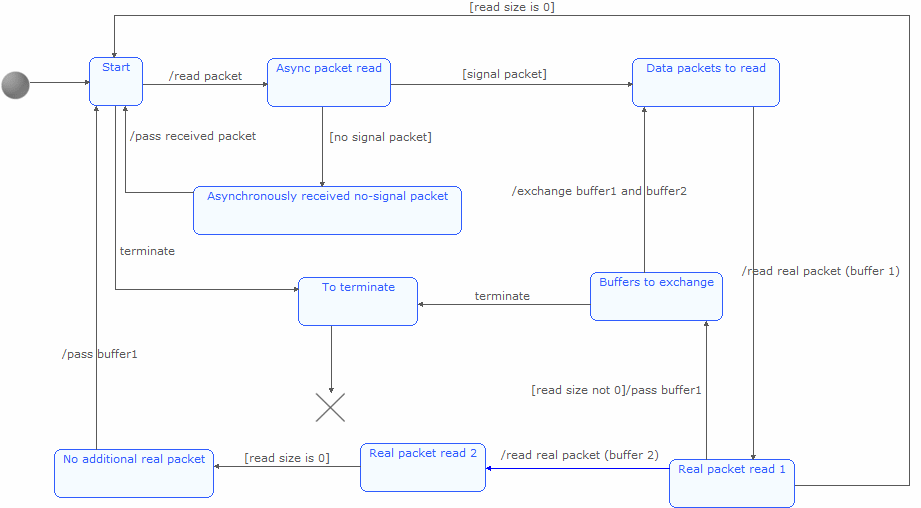
\includegraphics[width=130mm]{uml/GeolocationGarminWin_state_machine.png}

\section{HTML}

A visual explanation of the UTF-8 code is included as Excel file \verb|utf8.xlsx| in the \verb|doc| folder. If someone wants to create LaTeX code out of it, I'd be interested\ldots

\section{IO}

\subsection{CoroutineStream}

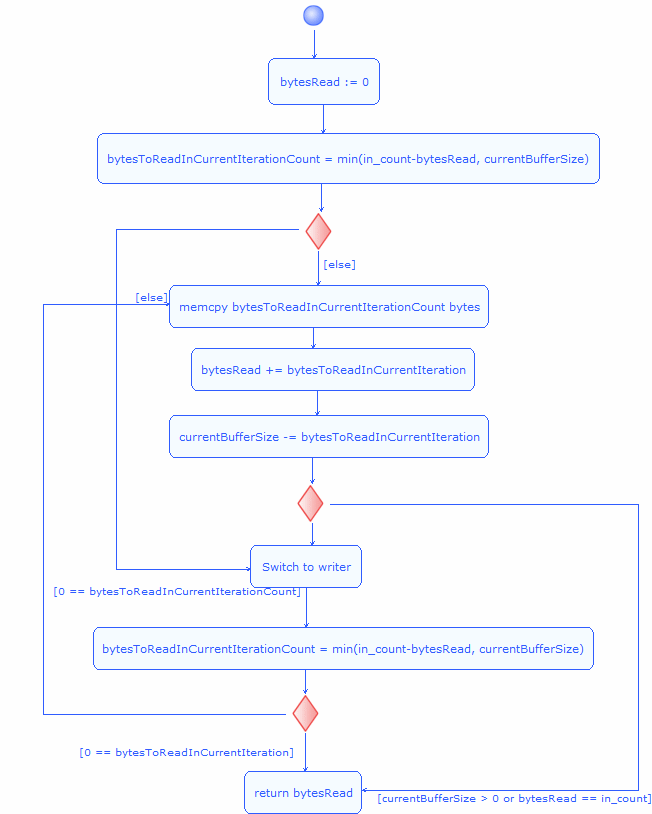
\includegraphics[width=130mm]{uml/CoroutineStream_read_activity.png}

Things that you should check to validate the model:

\begin{tabular}{| l | l | p{4.9cm} | l |}
\hline
\# & Call & Remark & Desired action \\
\hline
\hline
  1 & \texttt{read(0)} & & Switch coroutine \\
\hline
\hline
  2 & \texttt{read(in\_count)} & $\texttt{in\_count} > 0$ and $\texttt{in\_count} < \texttt{currentBufferSize}$ & Don't switch coroutine \\
\hline
  3 & \texttt{read(in\_count)} & $\texttt{in\_count} > 0$ and $\texttt{in\_count} == \texttt{currentBufferSize}$ & Don't switch coroutine \\
\hline
  4 & \texttt{read(in\_count)} & $\texttt{in\_count} > 0$ and $\texttt{in\_count} > \texttt{currentBufferSize}$ & Switch coroutine \\
\hline
\end{tabular}
\\

Why do we require the function to behave like this?

Lets go through the cases:

\paragraph{Case 1} \texttt{read(0)} is actually intended for switching the coroutine

\paragraph{Case 2} If we want to read data and data is available we can simply read it -- this should be obvious

\paragraph{Case 3} The reason why we don't switch the coroutine in case \texttt{in\_count} $>$ 0 and \texttt{in\_count} $==$ \texttt{currentBufferSize} is that we want to handle data as soon as possible. Additionally if we would the code of the reader coroutine in ``PipeStream example 2 -- reader coroutine'' (Listing \ref{lst:pipestream3}) would never reach the test.

\paragraph{Case 4} This should be obvious: if there is not enough data available we have to switch the coroutine

\subsection{PipeStream}

We have to store whether we already read data 

Imagine the following example:

\begin{lstlisting}[caption=PipeStream example 1 -- writer coroutine, label=lst:pipestream0]
pipeStreamInit(&state, ...);

// we write nothing

// Now we terminate to call the other coroutine
pipeStreamWrite(&state, NULL, 0);
\end{lstlisting}

\begin{lstlisting}[caption=PipeStream example 1 -- reader coroutine, label=lst:pipestream1]
size_t readCount = 0;
uint8_t buffer;

while (pipeStreamRead(&state, &buffer, 1))
	readCount++;

test(0 == readCount);
\end{lstlisting}

When calling \lstinline|pipeStreamWrite(&state, NULL, 0);| we switch to the other coroutine. Here we will call \lstinline|pipeStreamRead(&state, &buffer, 1);| This will switch back to the writer coroutine. The line \lstinline|test(READ_SIZE == readCount);| gets never called.

We can not easily change the source code since the following one is correct:

\begin{lstlisting}[caption=PipeStream example 2 -- writer coroutine, label=lst:pipestream2]
uint8_t buffer[2];

pipeStreamInit(&state, ...);

write(&state, buffer, 2);

// Now we terminate to call the other coroutine
pipeStreamWrite(&state, NULL, 0);
\end{lstlisting}

\begin{lstlisting}[caption=PipeStream example 2 -- reader coroutine, label=lst:pipestream3]
size_t readCount = 0;
uint8_t buffer;

while (pipeStreamRead(&state, &buffer, 1))
	readCount++;

test(2 == readCount);
\end{lstlisting}

So we solve this problem by switching to the other coroutine when initializing the PipeStream.

\subsection{BidirectionalStream}

The same examples as for ByteStream also apply to BidirectionalStream.

\part{Bits and pieces}

\chapter{Web standards}

\section{Sources for web standards}

\subsection{Crypto}

\subsubsection{SHA-1 and SHA-2}

\paragraph{Where can I get information concerning SHA-1 and SHA-2?}
\begin{itemize}
\item FIBS 180-3: \verb|http://csrc.nist.gov/publications/fips/fips180-3/fips180-3_final.pdf|
\item RFC 3174: \verb|http://www.apps.ietf.org/rfc/rfc3174.html|
\end{itemize}

\subsection{Graphics}

\subsubsection{GIF}

\paragraph{Where can I find the specification of GIF files?}
Look at \\
\verb|http://www.w3.org/Graphics/GIF/spec-gif87.txt| (GIF87A) and \\
\verb|http://www.w3.org/Graphics/GIF/spec-gif89a.txt| (GIF89A).

\subsubsection{JPEG}

\paragraph{Where can I get the ITU-T T.81 standard?} Under \verb|http://www.w3.org/Graphics/JPEG/| there is a link to \verb|http://www.w3.org/Graphics/JPEG/itu-t81.pdf|

\paragraph{Where can I get the ITU-T T.83 standard?} The authors of 101\_browser are not aware of a costless way that they are sure to be legal. So you will either have to pay or be on your own. :-(

Hint for adventurous people who don't fear legal consequences: search engines are a great invention. ;-)

\paragraph{Where can I obtain the test vectors for ITU-T T.83?} Under \\
\verb|http://www.itu.int/net/itu-t/sigdb/speimage/Tseries-s.htm|
there is a link to
\verb|http://www.itu.int/net/itu-t/sigdb/speimage/ImageForm-s.aspx?val=1010083|
where you can get the test vectors.

\paragraph{Where can I obtain the test vectors for JBIG2?}

\verb|http://web.archive.org/web/20040625064451/http://www.ece.ubc.ca/spmg/jbig2/bitstreams/main.html|

These files are also mirrored at \verb|http://jbig2dec.sourceforge.net/ubc/main.html|

Further information about JBIG2 test vectors can be found at \verb|http://jbig2dec.sourceforge.net/|

\subsubsection{PNG}

\paragraph{Where can I find the specification for PNG?} \verb|http://www.w3.org/TR/PNG/|

\paragraph{Where can I find a test suite for PNG?}

Under \verb|http://www.libpng.org/pub/png/pngmisc.html| there are links to various test images; among them the official test suite \verb|http://www.schaik.com/pngsuite/| that is also mirrored at \verb|http://www.libpng.org/pub/png/pngsuite.html|.

\subsection{Markup languages}

\subsubsection{HTML/HTML5/Web Applications 1.0 etc.}

\paragraph{Where do I get an overview about the various standards?} ~ \\
\verb|http://wiki.whatwg.org/wiki/FAQ#What_are_the_various_versions_of_the_spec.3F|

Additional URLs:
\begin{itemize}
\item DOM Core \verb|http://dvcs.w3.org/hg/domcore/raw-file/tip/Overview.html|
\item DOM Range \verb|http://html5.org/specs/dom-range.html|
\end{itemize}

\subsubsection{WPF}

\paragraph{Where can I find the specification of WPF?} ~ \\
\verb|http://msdn.microsoft.com/en-us/library/ff629155(PROT.10).aspx|

\paragraph{Where can I find a test suite for WPF?} ~ \\
\verb|http://blogs.msdn.com/b/llobo/archive/2010/07/07/xaml-compliance-suite-v1.aspx|

\subsection{Programming}

\subsubsection{ECMAScript}

\paragraph{Where can I find the specifications of ECMAScript?} ~ \\
On \verb|http://www.ecmascript.org/| (or more exactly: \\
\verb|http://www.ecma-international.org/publications/standards/Ecma-262.htm| \\
Deeplink: \verb|http://www.ecma-international.org/publications/files/ECMA-ST/ECMA-262.pdf|).

\subsection{Video}

\subsubsection{Matroska}

\paragraph{Where can I find the specification of Matroska?} ~ \\
On \verb|http://matroska.org/technical/specs/index.html|

A first explanation (but no reference): \verb|http://matroska.org/files/matroska.pdf|

\end{document}